\documentclass[]{article}
\usepackage[utf8]{inputenc}
\usepackage{graphicx}
\usepackage{float}
\usepackage[T1]{fontenc}
\usepackage{cite}

\usepackage{url}
\usepackage[portuguese]{babel}
\usepackage[T1]{fontenc}

\newcommand\x[1]{\discretionary{#1}{#1}{#1}}

\graphicspath{ {figs/} }
\title{Predizendo ní­veis de pobreza utilizando imagens de satélites e formulários socioeconômicos}
\author{João Pedro Donaire Albino }
\date{Junho 2019}

\begin{document}


\begin{center}
	\renewcommand{\baselinestretch}{1}
\end{center}

\vspace*{1cm}

\begin{center}
	\textbf{Relatório final de Iniciação Científica}
	
	\vspace*{1cm}
	
	\renewcommand{\baselinestretch}{2}
	\bf {\huge \sc Predizendo níveis de pobreza utilizando imagens de satélites e formulários socieconômicos.}
	\renewcommand{\baselinestretch}{1}
	
\end{center}

\vspace*{2.0cm}

\begin{center}
	
	\large João Pedro Donaire Albino
	
	\vspace*{1.0cm}
	
	\large Orientador:
	\large Prof. Dr. Clayton Pereira
	
	\vspace*{0.5cm}
	
	Departamento de Computação, Faculdade de Ciências, Universidade Estadual Paulista Júlio de Mesquita Filho\\
	Av. Eng. Luiz Edmundo Carrijo Coube, 14-01 - Vargem Limpa, CEP 17033-360 - Bauru - SP.
	
\end{center}

\vspace*{2.0cm}

\centerline{\large \today}

\newpage

\section{Introdução}
\label{s.introducao}

A pobreza é uma das chagas complexas e importantes de nossa sociedade atualmente, pois se trata de um problema dificilmente controlado e trabalhado por métodos efetivos de combate ~\cite{ref_pobreza1}. Atrelado a isso também temos uma escassez de dados relevantes que possam mensurar com consistência indicadores de qualidade de vida e de poder aquisitivo da população. Esses dois fatores desencadeiam um notável esforço para mapear e diagnosticar o cenário da pobreza em determinadas regiões, assim perpetuando o problema da má distribuição de renda no país \cite{ref_ma_distribuicao}.

Por outro lado, atualmente, a gestão de dados no Brasil melhorou, porém ainda temos [PROCURAR SOBRE GESTÃO]. 

TEXTO

\subsection{Origem do Tema}
A necessidade da aplicação mapeamento sobre pobreza sempre foi algo necessário e a aplicação de métodos para diminuir custos é algo que pode auxiliar na sua realização. Por tanto, trazer métodos tecnológicos para é algo que poderia auxiliar em tal tema, facilitando a aplicação de recursos financeiros, normalmente governamentais, para problemas que de fato poderiam ser combatidos com investimentos.

\subsection{Justificativa da Pesquisa}
Em setembro de 2015, líderes dos 193 países membros da Organização das Nações Unidas (ONU) aprovaram um plano global de desenvolvimento sustentável, com o objetivo de melhorar os indicadores econômicos, sociais e ambientais para as próximas gerações\cite{ref_nacoes}. Algo relevante para a proposta de pesquisa em questão é averiguar que a primeira dessas metas configura-se em eliminar todas as formas de pobreza no mundo. Essa decisão foi tomada ao levar em consideração que cerca de 705,5 milhões de pessoas vivem atualmente na extrema pobreza \cite{ref_extrema_pobreza}. 

Para exemplificar através de dados locais, uma das principais dificuldades do Brasil reside em direcionar recursos para as população mais pobre \cite{ref_lazarotto}. Mesmo que através de formulários e pesquisas se torna possível identificar regiões com altos índices de pobreza, sofremos em obter dados relevantes que mensuraram, indicam e agrupam regiões por níveis de renda ou outras indicadores importantes.

Outro ponto relevante para se levar em consideração na proposta do trabalho diz respeito à quantidade de investimentos necessários para realizar uma pesquisa intensiva bem esclarecedora sobre indicadores de pobreza. Se levarmos em consideração países que não possuem recursos abundantes, obter dados relevantes se torna algo difícil. Segundo o próprio Instituto Brasileiro de Geografia e Estatística (IBGE), o orçamento do Censo de 2010 realizado no país fora calculado em R\$ 1,677 bilhão \cite{ref_IBGE}.

Analisando tais fatos, chega-se em uma investida para inferir indicadores precisos utilizando dados \textit{open-source} gratuitos já disponíveis na \textit{Internet}. Esse é um dos tópicos que a Tecnologia de Dados que há algum tempo vem sendo trabalhado e será tratado dentro desta pesquisa.

\subsection{Formulação do problema}
É possível correlacionar intensidade luminosa com riqueza econômica utilizando dados open-source e Machine Learning?

\subsection{Objetivos da Pesquisa}
A pesquisa tinha como escopo principal criar um sistema utilizando Python e R totalmente automatizado para extrair, estruturar, carregar e classificar imagens de satélites noturnos do Estado de São Paulo, sendo estes de origem open-source.

\subsection{Estrutura do Trabalho}
O capítulo 1 discute-se sobre a introdução da pesquisa e objetivos da mesma. Nos dois seguintes trabalha-se apoio teórico e bibliográfico sobre o tema bem como metodologias de pesquisa aplicadas ao mesmo. O capítulo 4 apresenta alguns dados coletados no desenvolvimento da pesquisa e o 5, por sua vez, as considerações finais sobre o desenvolvimento da pesquisa.

\section{Rerenferencial Teórico}
\label{s.referencia_teorico}

\subsection{Kmeans}

\subsection{SVM}

\section{Metodologia}
Toda a pesquisa foi baseada em 4 macro principais estágios de análise de dados: Extração, Estruturação, Classificação e Predição. Além disso, para detalhar tem-se 7 microestágios correspondentes.

Divide-se a pesquisa em:
\begin{enumerate}
	
	\item Extração de dados de uma origem open-source;
	
	\item Estruturação das imagens no formato PGM;
	
	\item Extração dos dados para uma planilha CSV;
	
	\item Estruturação dos dados socioecônomicos abertos [CONFIRMAR COMO CHAMAM DADOS ABERTOS];
	
	\item Concepção de classes baseados nos dados socioeconômicos;
	
	\item Predição com modelos de Machine Learning;
	
	\item Validação dos dados.
	
\end{enumerate}

Na primeira etapa da pesquisa foi necessário um modelo para obter elementos em imagens de satélite e sócioeconômicos. A linguagem escolhida desde o início do projeto para construir o sistema foi o Python em conjunto com o R. Tal escolha baseou-se na alta demanda da mesma atualmente e na quantidade de bibliotecas que auxiliam nos estudos de Machine Learning. Foram utilizados o seguinte banco de dado imagético: National Geophysical Data Center Nighttime Lights Time Series para compor as imagens de dados de satélites noturnos. Além disso, todas as imagens foram computadas em TIFF, por padrão da origem. Porém foram convertidas para PGM como falaremos posteriormente.

Para o segundo momento, foi necessário definir padronização dos formatos dos dados. Nessa etapa, foi estabelecido que seria utilizado PGM como dados de imagem, PORQUE [EXPLICAR AQUI]. Além disso, todos os dados seriam estruturados em planilhas csv, por conta de [EXPLICAR MOTIVAÇÃO AQUI. PROCURAR ARTIGO NA NET].

Para o terceiro momento, extrai-se a intensidade luminosa dos mapas noturnos colocados em CSV com 198 pixels [CONFIRMAR CONVERSÃO]. Nesse caso, cada imagem é convertida em uma linha com 198 colunas. Depois disso foi necessário criar classes dos dados. Para tanto, usaram-se os índices de Produto Interno Bruto (PIB) de 2010 obtidos na pesquisa do IBGE, e foram auferidos classes utilizando KMEANs e PIB para comparar com o classificador SVM.
Por fim, utilizamos o SVM baseado em 3 classes: menor, médio e maior. Ambas se baseiam em cidades com mínimo, médio e máximo das cidades de São Paulo.


Na primeira etapa da pesquisa é necessário um modelo bem treinado e preparado para identificar elementos em imagens de satélite, possibilitando no final um sistema útil para identificação de níveis de pobreza. Portanto, em uma primeira instância, deve-se utilizar um modelo de CNN treinado a fim de identificar características básicas de imagens. A linguagem escolhida para construir o sistema será o Python. Tal escolha baseia-se na alta demanda da mesma atualmente e na quantidade de bibliotecas que auxiliam nos estudos de \textit{Machine Learning}.

Para o segundo momento, deve-se desenvolver uma aprendizagem em relação a imagens de mapas diurnos e noturnos. Primeiro, extrai-se a intensidade luminosa do mapas diurnos para, em seguida, identificar a correlacionar essa aprendizagem às imagens de mapas diurnos. 

Serão utilizados os seguintes bancos de dados imagéticos: Mapas de satélites diurnos (Google Static Maps API) e de satélites noturnos (National Geophysical Data Center, Version 4 DMSP-OLS Nighttime Lights Time Series).

Em um terceiro momento, será necessário correlacionar as atribuições possíveis com os mapas aos dados socioeconômicos já obtidos pelos questionários. Para a análise desses dados, a pesquisa utilizará dados de formulários brasileiros de pesquisa de consumo fornecidos por instituições que fornecem dados abertos, como o próprio IBGE. Por fim, o produto final do projeto   

Por fim, será feito uma avaliação final dos dados obtidos. Será avaliado se a classificação pelas imagens de fato condizem com os dados brutos obtidos pelos formulários.

\section{Apresentação e Análise de dados}
No primeiro mês de projeto, foi estruturada a origem dos dados que seriam utilizados, para que pudesse assim ser definido modelo e classificação dos dados. Para tanto, todas as procuras foram guiadas em encontrar dados abertos. Na pesquisa [CITA PESQUISA DE STANDFORD], eles utilizaram dados do portal National Geophysical Data Center para predizer dados da Nigéria e Uganda. A justificativa inicial foi vinculada às facilidades e qualidades dos dados do portal, portanto, partiu-se do mesmo pressuposto no projeto. E a escolha beneficiou em automatizar o processo da obtenção grande quantidades dos dados.

IMAGEM MOSTRANDO DADO SENDO OBTIDO E SALVO NAS PASTAS

Nos outros meses 2, foi focada a criação de algoritmos para realizar tal tarefas. A funcionalidade básica do algoritmo se reunimia na imagem seguinte. 

FLUXOGRAMA MOSTRANDO A OBTENÇÃO DOS DADOS

Primeiramente, esperamos obter dados de 10 km por 10 km em arquivos TIFF. A escolha da quilometragem assegura que a localização obtida no mapa estivesse na análise. A contabilização realizada foi uma avaliação de um ponto como:
\begin{enumerate}
	
	\item km lon = 10*(360/23903.297);
	
	\item km lat = 10*(360/40075.00)
	
\end{enumerate}

Realizou-se a obtenção de 3.075 imagens realizando o download baseado nas máximas e mínimas longitudes e latitudes do estado de Estado de São Paulo. Por fim, foram obtidos dados de todos satélites, porém utilizaram-se imagens apenas do ano de 2010 os satélites. Obtidos os dados, foi escolhido convertê-los para uma análise de pixels em 198.
Depois de elencadas as imagens, foi preciso rotular os dados com as referentes cidades. Para tanto utilizamos a API do Google Maps, com ele foi possível enviar as latitutes e longitudes para obter o nome da área referente.Com isso, foi possível identificar XX de XX nos municípios do estado de São Paulo.
Após tal fato, foi possível escolher a maneira mais aconselhável para predizer os dados. Primeiramente, elencaram-se em duas classes para usar como dados rotulados. A primeira classe foi escolhida baseada na classificação World Bank (https://blogs.worldbank.org/opendata/new-country-classifications-income-level-2017-2018, a qual divide como PIB:
- Baixo: Renda menor ou igual a U\$3955
- Médio: Renda entre U\$3955 e U\$12235
- Alto: Maior ou igual a U\$12235
Com essa classificação foram obtidos os seguintes dados:

IMAGEM COM OS DADOS DA CLASSIFICAÇÃO COM PIB

Na segunda classe procurou-se rotular os dados otimizando com um classificador. KMEANs trouxe as seguintes classes para análise:

MOSTRAR DADOS COM O KMEANS

Com os dados rotulados, utilizou-se o SVM para classificar as imagens auferidas. Essas 3 classes baseadas na quantidade de pixels, estabelecemos 3 cidades que seriam usadas como base para o classificador. Do mais baixo para o maior tivemos:
- Menor = Lucianópolis com uma soma de 0 pixels;
- Médio = Pirangi com 4558.0 pixels;
- Alto = São Paulo com a soma de 114735.0 pixels.

O resultado dessa classificação foi conferido em conjunto com os outros dados rotulados. Por final, foi possível o resultado de 68,74\% utilizando KMEANs e 54\% utilizando os classificadores da ONU.



\section{Cronograma}
O objetivo desta sessão é formalização do plano de distribuição das etapas do projeto. O projeto tem a previsão de um ano de realização. A Tabela \ref{f.cronograma} apresenta esse cronograma.

\begin{figure}[!ht]
	\centerline{
		\begin{tabular}{c}
			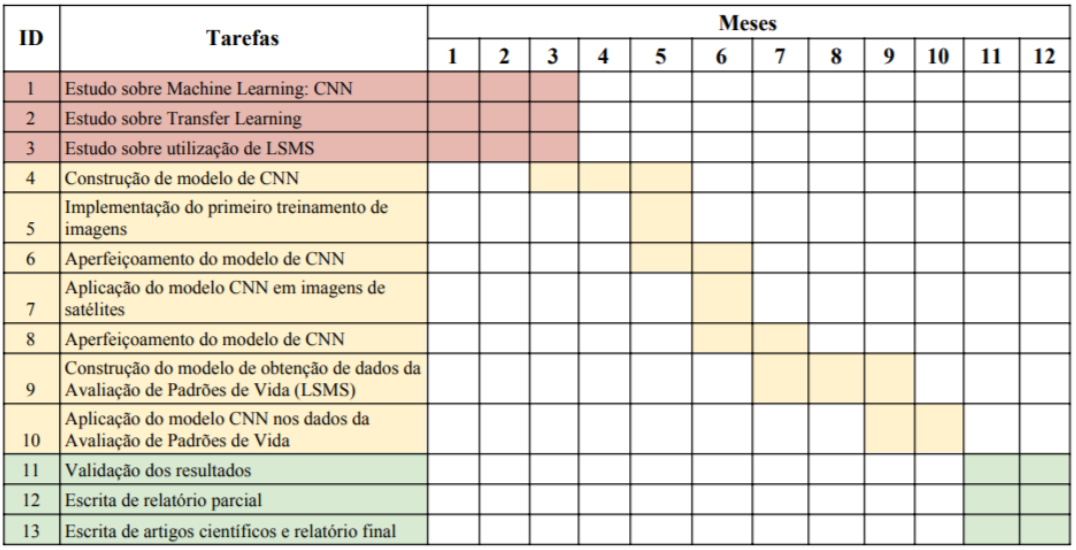
\includegraphics[width=12cm]{figs/cronograma.png}\\
		\end{tabular}
		}
		
		
		
		\caption{Cronograma de atividades da presente proposta}		
		\label{f.cronograma}
	
\end{figure}

\section{Conclusões}
No final deste período de pesquisa, considerando a quantidade de dados obtidos, os modelos aplicados e a acurácia auferida, avalia-se com um bom resultado da mesma.
Primeiramente, foram utilizados cerca de 3.075 itens de 10 km x 10 km no formato PGMs , algo que compactua com cerca de 644 cidades do estado de São Paulo, correspondendo XX\% de todas. Já em um segundo momento, estruturaram-se os dados de maneira automatizada assim possibilitando utilizar dois classificadores de dados e utilizar ao menos um método de predição. Por fim, alcançando cerca de XX\% de correspondência dos dados.

COLOCAR FIGURA MOSTRANDO RESULTADOS

Porém, pode-se dizer que a pesquisa possui alguns pontos de melhora. Primeiramente, na utilização mais teórica dos dados de base, trazendo conhecimentos socioeconômicos mais refinados para então usar outros índices de desempenho econômico que iriam além do PIB.
Além disso, seria muito importante utilizar mais de uma método de Machine Learning para validar os resultados esperados. Pensa-se em continuar com os estudos para implementação da OPF (COLOCAR REFERÊNCIA), por exemplo, que provou-se ser aconselhável para uso de dados como PGM.
Por fim, 


%----------------------------------------------------------------------------
% Bibliography

\bibliographystyle{./IEEEtran}
\bibliography{refs}



%----------------------------------------------------------------------------

\end{document}
